\documentclass[9pt]{article}
\usepackage{fancyhdr, titling, graphicx, extsizes, hyperref}
\pagestyle{fancy}

\author{Ben Green}
\title{Intro to Data Science Project Proposal}

% put name and page number in header
\fancyhead[L]{Ben Green}
\fancyhead[R]{Project Proposal}

\begin{document}

\textbf{TomTom meets TripAdvisor - A Trip Itinerary Feedback Engine}

\section{Project Members}
I will be the only member of this project.

\section{Project Definition}
The concept is simple - input an itinerary of places to visit (for now, in Iceland) over the course of a day (or days), and provide feedback on each step in the schedule based on factors including, but not limited to:
	\begin{itemize}
	\item{Weather at locations along route}
	\item{Road conditions between said locations}
	\item{Visibility of Northern Lights (when taking into account overnight stays)}
	\item{Nearby concerts and/or sporting events (to fill time or become substitutes for rained-out trips to the beach)
	\item{Others who may be ride-sharing along a route on the itinerary}}
	\end{itemize}
and much, much more. With this kind of data, a prospective traveler (or even one who is already midway through their trip) can make sure their day in Iceland will go smoothly. If large gaps of free time are indicated (or if a desired event becomes impractical due to unforeseen conditions), the nearby area can be analyzed to bring up suitable events/tour sites that would fit well with the existing schedule.\\

Here is a sample custom Google map one might use as their itinerary for the purposes of this program:

\begin{center}
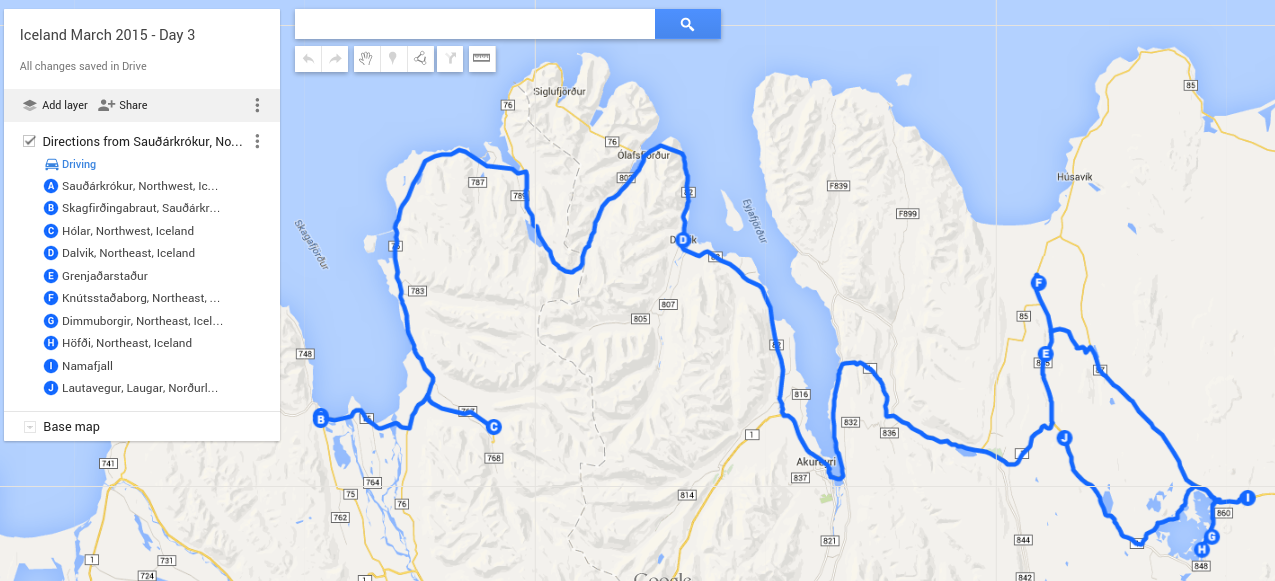
\includegraphics[keepaspectratio, scale=0.2]{map.png}
\end{center}

\section{Project Significance}
The project is of particular interest to me personally as I will be visiting Iceland over the next week - that aside, if this concept was applied to many countries, it would be very convenient for travelers to immediately receive feedback if an upcoming event becomes impractical, along with various alternative recommendations - not unlike the way your phone might recommend alternate routes if a roadblock appears while driving.

\section{Expected Difficulty \& Hypotheses}
To work well, this kind of suggestion engine needs to be tailored to the country it is designed for - things such as optimal Northern Lights viewing are specific to Iceland, and therefore indispensable to the design of this analyzer. In addition, a good algorithm to compare and contrast the relative 'benefits' of one location over another must be implemented. I predict that this algorithm will be the most difficult component of the project, as to function well it should dynamically adapt to the preferences of each individual user. As described below, most of the API work has been done already, so I shouldn't need to worry too much about that.\\

I searched around quite a bit, and didn't seem to find anything similar at all - sites such as Google Maps let you plan out an adventure via a custom route (and I plan to use that as the input to this suggestion engine), and sites such as TripAdvisor will recommend interesting destinations and hotels (and even weather data!), but I haven't come across any that combine the two to provide something quite like this.

\section{Key Components}
Naturally, the most significant data components will be the user's itinerary, the constantly-changing data regarding weather, road conditions, and other such factors to be applied to each location in real-time,and a database of additional commonly-visited locations in Iceland. This database will be used along with dynamically found concerts/events to provide recommendations to fill blocks of empty time. The algorithm and front-end will likely be in either Python or Java (probably the former). As data will all be clearly labeled, this is a supervised learning problem.

\section{Data Sources \& Conclusion}
Data for carpooling, road conditions, earthquakes, sports events, and concerts will be taken from the convenient APIs at \url{http://docs.apis.is}. This data is already (thankfully) clean.\\

\noindent{}Data for weather and Northern Lights viewings will be scraped from the Icelandic weather site \url{http://en.vedur.is}. This data will very likely require cleaning, although I have used the handy web scraper \url{http://import.io} before and it does an excellent job of minimizing the amount of collected junk data.\\

Implementing the dynamic algorithm to determine each location's 'recommendation level' is what I am most looking forward to learning about. Ideally, this will be shown in a format wherein it will provide relevant, useful results across a wide range of user preferences.

\end{document}